%!TEX TS-program = xelatex
%!TEX encoding = UTF-8 Unicode

\documentclass[12pt]{article}
\usepackage{geometry}
\usepackage{float}
\usepackage{amssymb}
\usepackage{tikz}
\usepackage{minted}
\usepackage{dirtree}
\usepackage{caption}
\usepackage{adjustbox}
\usepackage[font={small,it}]{caption}
\usepackage{ifxetex,ifluatex}
\usepackage{framed}
\usepackage[12pt]{moresize}
\usepackage{graphicx}
\graphicspath{{./images/}}

\usepackage{fancyhdr}
\setlength{\headheight}{25pt}
\pagestyle{fancy}
\fancyhf{}
\fancyhead[L]{\leftmark}
\fancyhead[R]{\rightmark}
\fancyfoot[C]{\thepage}

\usepackage{fontspec,xltxtra,xunicode,xeCJK}
\usepackage[
  colorlinks=true,
  linkcolor=blue,
  bookmarksnumbered=true,
  CJKbookmarks=true,
  bookmarksopen=true]{hyperref}

\newcommand{\mytitle}[1]{
  {\HUGE \bfseries #1}\par
}

\newcommand{\mysubtitle}[1]{
  {\emph{#1}}\par
}

\definecolor{titlepagecolor}{cmyk}{1,.60,0,.40}

\DeclareFixedFont{\titlefont}{T1}{ppl}{b}{it}{1.0in}

\newminted{sql}{
  autogobble,
  breaklines,
  frame=leftline,
  framerule=1.2pt,
  framesep=1em,
  linenos,
  fontsize=\footnotesize
}

\newminted{xml}{
  autogobble,
  breaklines,
  frame=leftline,
  framerule=1.2pt,
  framesep=1em,
  linenos,
  fontsize=\footnotesize
}

\newminted{bash}{
  autogobble,
  breaklines,
  frame=leftline,
  framerule=1.2pt,
  framesep=1em,
  linenos,
  fontsize=\footnotesize
}

%!TEX TS-program = xelatex
%!TEX r = UTF-8 Unicode
%!TeX root = manual.tex

% conditional for xetex or luatex
\newif\ifxetexorluatex
\ifxetex
  \xetexorluatextrue
\else
  \ifluatex
    \xetexorluatextrue
  \else
    \xetexorluatexfalse
  \fi
\fi
%
\ifxetexorluatex%
  \usepackage{fontspec}
  \usepackage{biolinum}
  \usepackage{libertineRoman} % or use \setmainfont to choose any font on your system
  \newfontfamily\quotefont[Ligatures=TeX]{Linux Libertine O} % selects Libertine as the quote font
\else
  \usepackage[utf8]{inputenc}
  \usepackage[T1]{fontenc}
  \usepackage{biolinum}
  \usepackage{libertineRoman} % or any other font package
  \newcommand*\quotefont{\fontfamily{LinuxLibertineT-LF}} % selects Libertine as the quote font
\fi

\newcommand*\quotesize{60} % if quote size changes, need a way to make shifts relative
% Make commands for the quotes
\newcommand*{\openquote}
   {\tikz[remember picture,overlay,xshift=-4ex,yshift=-2.5ex]
   \node (OQ) {\quotefont\fontsize{\quotesize}{\quotesize}\selectfont``};\kern0pt}

\newcommand*{\closequote}[1]
  {\tikz[remember picture,overlay,xshift=4ex,yshift={#1}]
   \node (CQ) {\quotefont\fontsize{\quotesize}{\quotesize}\selectfont''};}

% select a colour for the shading
\colorlet{shadecolor}{white}

\newcommand*\shadedauthorformat{\emph} % define format for the author argument

% Now a command to allow left, right and centre alignment of the author
\newcommand*\authoralign[1]{%
  \if#1l
    \def\authorfill{}\def\quotefill{\hfill}
  \else
    \if#1r
      \def\authorfill{\hfill}\def\quotefill{}
    \else
      \if#1c
        \gdef\authorfill{\hfill}\def\quotefill{\hfill}
      \else\typeout{Invalid option}
      \fi
    \fi
  \fi}
% wrap everything in its own environment which takes one argument (author) and one optional argument
% specifying the alignment [l, r or c]
%
\newenvironment{shadequote}[2][l]%
{\authoralign{#1}
\ifblank{#2}
   {\def\shadequoteauthor{}\def\yshift{-2ex}\def\quotefill{\hfill}}
   {\def\shadequoteauthor{\par\authorfill\shadedauthorformat{#2}}\def\yshift{2ex}}
\begin{snugshade}\begin{quote}\openquote}
{\shadequoteauthor\quotefill\closequote{\yshift}\end{quote}\end{snugshade}}


%!TEX TS-program = lualatex
%!TEX r = UTF-8 Unicode
%!TeX root = manual.tex

\newcommand\titlepagedecoration{%
\begin{tikzpicture}[remember picture,overlay,shorten >= -10pt]

\coordinate (aux1) at ([yshift=-15pt]current page.north east);
\coordinate (aux2) at ([yshift=-410pt]current page.north east);
\coordinate (aux3) at ([xshift=-4.5cm]current page.north east);
\coordinate (aux4) at ([yshift=-150pt]current page.north east);

\begin{scope}[titlepagecolor!40,line width=12pt,rounded corners=12pt]
\draw
  (aux1) -- coordinate (a)
  ++(225:5) --
  ++(-45:5.1) coordinate (b);
\draw[shorten <= -10pt]
  (aux3) --
  (a) --
  (aux1);
\draw[opacity=0.6,titlepagecolor,shorten <= -10pt]
  (b) --
  ++(225:2.2) --
  ++(-45:2.2);
\end{scope}
\draw[titlepagecolor,line width=8pt,rounded corners=8pt,shorten <= -10pt]
  (aux4) --
  ++(225:0.8) --
  ++(-45:0.8);
\begin{scope}[titlepagecolor!70,line width=6pt,rounded corners=8pt]
\draw[shorten <= -10pt]
  (aux2) --
  ++(225:3) coordinate[pos=0.45] (c) --
  ++(-45:3.1);
\draw
  (aux2) --
  (c) --
  ++(135:2.5) --
  ++(45:2.5) --
  ++(-45:2.5) coordinate[pos=0.3] (d);
\draw
  (d) -- +(45:1);
\end{scope}
\end{tikzpicture}%
}


\begin{document}

\begin{titlepage}
\begin{minipage}{0.8\linewidth}
  \vspace*{4cm}
  \begin{center}
    \noindent
    \mytitle{Evolutionary Database Design}
    \rule{\linewidth}{0.2ex}\par
    \mysubtitle{Pramod Sadalage \\ Martin Fowler \\ typeset by Justin
    Zhang}
  \end{center}
\end{minipage}
\null \vfill
\hfill
\begin{minipage}{0.55\linewidth}
  \begin{flushright}
    % \printauthor
  \end{flushright}
\end{minipage}
%
% \begin{minipage}{0.02\linewidth}
%   \rule{1pt}{260pt}
% \end{minipage}
\titlepagedecoration
\end{titlepage}

\newpage
\tableofcontents
% \newpage
% \listoffigures
% \newpage
% \listoftables
% \newpage
% \listoflistings

\newpage
This document is typesetted by \href{mailto:schnell18@gmail.com}{\emph{Justin
Zhang}} in \LaTeX\ for better screen reading experience. The authors of
this document are \emph{Pramod Sadalage} and \emph{Martin Fowler}. You
may read the document in its original form at
\href{https://www.martinfowler.com/articles/evodb.html}{https://www.martinfowler.com/articles/evodb.html}.

\newpage
\emph{
Over the last decade we've developed and refined a number of techniques
that allow a database design to evolve as an application develops. This
is a very important capability for agile methodologies. The techniques
rely on applying continuous integration and automated refactoring to
database development, together with a close collaboration between DBAs
and application developers. The techniques work in both pre-production
and released systems, in green field projects as well as legacy systems.
}

\newpage
\section{Evolutionary Database Design}

In the past decade, we've seen the rise of
\href{https://martinfowler.com/articles/newMethodology.html}{agile
methodologies}. Compared to their predecessors they change the demands
on database design. One of the most central of these demands is the idea
of evolutionary architecture. On an agile project you assume that you
cannot fix the requirements of the system up-front. As a result having a
detailed design phase at the beginning of a project becomes impractical.
The architecture of the system has to evolve through the various
iterations of the software. Agile methods, in particular
\href{https://martinfowler.com/articles/newMethodology.html#XpextremeProgramming}{extreme
programming (XP)}, have a number of practices that make this
evolutionary architecture practical.

When we and our Thoughtworks colleagues started doing agile projects, we
realized that we needed to solve the problem of how to evolve a database
to support this evolution of architecture. We began around 2000 with a
project whose database ended up with around 600 tables. As we worked on
this project we developed techniques that allowed to change the schema
and migrate existing data comfortably. This allowed our database to be
completely flexible and evolvable. We described these techniques in an
earlier version of this article, a description that's inspired other
teams and toolsets. Since then we've used and further developed these
techniques on hundreds of projects world-wide, from small teams to large
multi-national programs of work. We've been long intending to bring this
article up to date, and now we've had the chance to give it a proper
refresh.

\newpage

\section{Jen implements a new story}

To get a feel for how all of this works, lets outline what happens when
a developer (Jen) writes some code to implement a new user story. The
story states that the user should be able to see, search, and update the
location, batch, and serial numbers of a product in inventory. Looking
at the database schema, Jen sees that currently there's no such fields
in the inventory table, just a single \verb=inventory_code= field which
is the concatenation of these three fields. She has to take this single
code and split it into three separate fields: \verb=location_code=,
\verb=batch_number= and \verb=serial_number=.

Here's the steps she'll need to go through:

\begin{itemize}
  \item Add new columns to the inventory table in the existing schema
  \item Write a data migration script to split data from the existing
    \verb=inventory_code= column updating the \verb=location_code=,
    \verb=batch_number= and \verb=serial_number= columns.
  \item Change the application code to use the new columns
  \item Change any database code, such as views, stored procedures and
    triggers, to use the new columns
  \item Change any indexes based on the \verb=inventory_code= column
  \item Commit this database migration script and all the application
    code changes to the version control system
\end{itemize}

To add new columns and migrate the data, Jen writes a SQL migration
script that she can run against the current schema. This will both
change the schema and also migrate all the existing data in the
inventory.

\begin{sqlcode}
ALTER TABLE inventory ADD location_code VARCHAR2(6) NULL;
ALTER TABLE inventory ADD batch_number VARCHAR2(6) NULL;
ALTER TABLE inventory ADD serial_number VARCHAR2(10) NULL;

UPDATE inventory SET location_code = SUBSTR(product_inventory_code,1,6);
UPDATE inventory SET batch_number = SUBSTR(product_inventory_code,7,6);
UPDATE inventory SET serial_number = SUBSTR(product_inventory_code,11,10);

DROP INDEX uidx_inventory_code;

CREATE UNIQUE INDEX uidx_inventory_identifier
  ON inventory (location_code,batch_number,serial_number);

ALTER TABLE product_inventory DROP COLUMN inventory_code;
\end{sqlcode}

Jen runs this migration script on a local copy of database on her
machine. She then proceeds to update the application code to use these
new columns. As she does this she runs the existing test suite against
this code to detect any changes in the application's behavior. Some
tests, those that relied on the combined column need to be updated. Some
tests may need to be added. Once Jen has done all this, and the
application has all its tests green on her machine, Jen pushes all her
changes to the shared project version control repository - which we call
the mainline. These changes include the migration scripts and the
application code changes.

If Jen isn't too familiar with making this change, she's fortunate that
it's a common one to make to a database. So she can look up it the
\href{https://martinfowler.com/books/refactoringDatabases.html}{database
refactoring book}, there's also a
\href{http://databaserefactoring.com/SplitColumns.html}{summary online}.

Once the changes are in mainline they will be picked up by the
\href{https://martinfowler.com/articles/continuousIntegration.html}{Continuous
Integration} server. It will run the migration scripts on the mainline
copy of the database, and then run all the application tests. If all is
green, this process will be repeated across the whole
\href{https://martinfowler.com/bliki/DeploymentPipeline.html}{Deployment
Pipeline}, including QA and Staging environments. The same code finally
is run against production, now updating the live database's schema and
data.

A small user story like this has only a single database migration,
larger stories are often broken down into several separate migrations
for each change to the database. Our usual rule is to make each database
change as small as possible. The smaller it is, the easier it is to get
right, and any errors are quick to spot and debug. Migrations like this
compose easily, so it's best to do many small ones.


\section{Dealing with Change}

As agile methods have spread in popularity in the early 2000s, one of
their most obvious characteristics is their towards change. Before they
appeared on the scene most of the thinking about software process was
about understanding requirements early, signing off on these
requirements, using the requirements as a basis for design, signing off
on that, and then proceeding with construction. This is a plan-driven
cycle, often referred to (usually with derision) as the waterfall
approach

Such approaches look to minimize changes by doing extensive up-front
work. Once the early work is done, changes cause significant problems.
As a result such approaches run into trouble if requirements are
changing, and requirements churn is a big problem for such processes.

Agile processes approach change differently. They seek to embrace
change, allowing changes to occur even late in a development project.
Changes are controlled, but the attitude of the process is to enable
change as much as possible. Partly this is in response to the inherent
instability of requirements in many projects, partly it is to better
support dynamic business environments by helping them change with the
competitive pressures.

In order to make this work, you need a different attitude to design.
Instead of thinking of design as a phase, which is mostly completed
before you begin construction, you look at design as an on-going process
that is interleaved with construction, testing, and even delivery. This
is the contrast between planned and evolutionary design.

One of the vital contributions of agile methods is that they have come
up with practices that allow evolutionary design to work in a controlled
manner. So instead of the common chaos that often happens when design
isn't planned up-front, these methods provide techniques to control
evolutionary design and make them practical.

An important part of this approach is iterative development, where you
run the entire software life-cycle many times during the life of a
project. Agile processes run complete life cycles in each iteration,
completing the iteration with working, tested, integrated code for a
small subset of the requirements of the final product. These iterations
are short, anywhere from a few hours to a couple of weeks, more skillful
teams use shorter iterations.

While these techniques have grown in use and interest, one of the
biggest questions is how to make evolutionary design work for databases.
For a long time, people in the database community considered database
design as something that absolutely needs up-front planning. Changing
the database schema late in the development tended to cause wide-spread
breakages in application software. Furthermore changing a schema after
deployment resulted in painful data migration problems.

Over the course of the last decade and half we've been involved in many
large projects that have used evolutionary database design and made it
work. Some projects involved more than 100 people in multiple sites
world-wide. Others involved over half-million lines of code, over 500
tables. Some had multiple versions of the application in production and
applications that needed 24*7 uptime. During these projects we have seen
iterations of a month and 1 week duration, shorter iterations worked
better. The techniques we describe below are the ones that we used to
make this work.

Since the early days we have tried to spread these techniques over more
of our projects, gaining more experience from more cases and now all our
projects use this approach. We've also found inspiration, ideas, and
experience from other agile practitioners.

\subsection{Limitations}

Before we dive into the techniques, it's important to state that we
haven't solved all the problems of evolutionary database design.

We have had projects with hundreds of retail stores having their own
database, all of which need to upgraded together. However we haven't yet
explored the situation where there is a lot of customization on such a
large group of sites. An example might be a small business application
that allows customization of the schema, deployed into thousands of
different small companies.

Increasingly we are seeing people use multiple schemas as part of a
single database environment. We've worked with projects using a handful
of schemas like this, but haven't yet cranked this up to tens or
hundreds of schemas. This is a situation that we anticipate having to
deal with in the next few years.

We don't consider these problems to be inherently unsolvable. After all
when we wrote the original version of this article we hadn't solved the
problems of 24*7 uptime or integration databases. We found ways to deal
with those, and expect we'll push the limits of evolutionary database
design further too. But until we do, we won't claim we can solve such
problems.

\section{The Practices}
Our approach to evolutionary database design depends on several important practices.

\subsection{DBAs collaborate closely with developers}

One of the tenets of agile methods is that people with different skills
and backgrounds need to collaborate very closely together. They can't
communicate mainly through formal meetings and documents. Instead they
need to be out talking with each other and working with each other all
the time.Everybody is affected by this: analysts, PMs, domain experts,
developers... and DBAs.

Every task that a developer works on potentially needs a DBA's help.
Both the developers and the DBA need to consider whether a development
task is going to make a significant change to the database schema. If
so, the developer needs to consult with the DBA to decide how to make
the change. The developer knows what new functionality is needed, and
the DBA has a global view of the data in the application and other
surrounding applications. Many times developers have visibility into the
application they are working on and not necessarily into all the other
upstream or downstream dependencies on the schema. Even if it's a single
database application, there could be dependencies in the database that a
developer isn't aware of.

At any time a developer can call on the DBA and ask to pair to sort out
a database change. By pairing, the developer learns about how the
database works, and the DBA learns the context of the demands on the
database. For most changes it's up to the developers to call on the DBA
if they are concerned about the database impact of changes. But DBAs
also take initiative. When they see stories that they think are likely
to have a significant data impact, they can seek out the developers
involved to talk through the database impact. DBAs can also review the
migrations as they get committed into version control. While it's
annoying to reverse a migration, we again gain from each migration being
small, which makes it easier to reverse.

To make this happen the DBA has to make herself approachable and
available. She needs to make it easy for a developer to just pop over
for a few minutes and ask some questions, maybe on the slack channel or
hipchat room or whatever communication medium the developers are using.
When setting up the project space, make sure the DBAs and developers sit
close to each other so they can easily get together. Ensure that DBAs
are told about any application design sessions so they can pop in
easily. In many environments we see people erecting barriers between the
DBA and application development functions. These barriers must come down
for an evolutionary database design process to work.

\subsection{All database artifacts are version controlled}

Developers benefit a lot from using version control for all their
artifacts: application code, unit and functional tests, and other code
such as build scripts, and puppet or chef scripts used to create an
environment.

\begin{figure}[H]

    \dirtree{%
    .1 .
    .1 buildscripts.
    .1 db.
    .2 BaseSchema.
    .2 DataDictionary.
    .2 DataModel.
    .2 Installation.
    .2 Migration.
    .2 PerformanceLoad.
    .2 ReferenceData.
    .2 SampleData.
    .2 Scripts.
    .2 StoredProcedures.
    .2 Tools.
    .2 Triggers.
    .1 lib.
    .1 puppet.
    .1 src.
    .1 test.
    .1 webapp.
    }
  \caption{All database artifacts are in version control along with other project artifacts}
  \label{fig:db-artifact}
\end{figure}

Similarly all the database artifacts should be in version control, in
the same repository that's being used by everyone else. The benefits for
this are:

\begin{itemize}
  \item There's only one place to look, making it easier for anyone on the project to find things.
  \item Every change to the database is stored, allowing easy audit if
    any problems occur. We can trace every deployment of the database to
    the exact state of the schema and supporting data.
  \item We prevent deployments where the database is out of sync with
    the application, which leads to errors retrieving and updating data.
  \item We can easily create new environments: for development, testing, and indeed production. Everything needed to create a running version of the software should be in a single repository, so it can be quickly checked out and built.
\end{itemize}

\subsection{All database changes are migrations}

In many organizations we see a process where developers make changes to
a development database using schema editing tools and ad-hoc SQL for
standing data. Once they've finished their development task, then DBAs
compare the development database to the production database and make the
corresponding changes to the production database when promoting the
software to live. But doing this at production time is tricky as the
context for the changes in development is lost. The purpose of the
changes needs be understood again, by a different group of people.

To avoid this we prefer to capture the change during development, and
keep the change as a first class artifact that can be tested and
deployed to production with the same process and control as changes to
application code. We do this by representing every change to the
database as a database migration script which is version controlled
together with application code changes. These migration scripts include:
schema changes, database code changes, reference data updates,
transaction data updates, and fixes to production data problems caused
by bugs.

Here is a change adding \verb=min_insurance_value= and
\verb=max_insurance_value= to the \verb=equipment_type= table, with some
default values.

\begin{sqlcode}
ALTER TABLE equipment_type ADD(
  min_insurance_value NUMBER(10,2),
  max_insurance_value NUMBER(10,2)
);

UPDATE equipment_type SET
          min_insurance_value  =  3000,
          max_insurance_value = 10000000;
This change adds some standing data to the location and equipment_type tables.

-- Create new warehouse locations #Request 497
INSERT INTO location (location_code, name , location_address_id,
  created_by, created_dt)
VALUES ('PA-PIT-01', 'Pittsburgh Warehouse', 4567,
  'APP_ADMIN' , SYSDATE);
INSERT INTO location (location_code, name , location_address_id,
  created_by, created_dt)
VALUES ('LA-MSY-01', 'New Orleans Warehouse', 7134,
  'APP_ADMIN' , SYSDATE);

-- Create new equipment_type #Request 562
INSERT INTO equipment_type (equipment_type_id, name,
  min_insurance_value, max_insurance_value, created_by, created_dt)
VALUES (seq_equipment_type.nextval, 'Lift Truck',
  40000, 4000000, 'APP_ADMIN', SYSDATE);
\end{sqlcode}

With this way of working, we never use schema editing tools such as
Navicat, DBArtisan or SQL Developer to alter schemas, nor do we ever run
ad hoc DDL or DML in order to add standing data or fix problems. Other
than updates to the database that occur due to the application software,
all changes are made by migrations.

Defining migrations as sets of SQL commands is part of the story, but in
order to apply them properly we need some extra things to manage them.

\begin{itemize}
  \item Each migration needs a unique identification.
  \item We need to track which migrations have been applied to the
    database
  \item We need to manage the sequencing constraints between the
    migrations. In the example above, we must apply the ALTER TABLE
    migration first, otherwise the second migration will fail to insert
    the equipment type.
\end{itemize}

We handle these demands by giving each migration a sequence number. This
acts as a unique identifier and ensures we can maintain the order that
they're applied to the database. When a developer creates a migration
she puts the SQL into a text file inside a migrations folder within the
project's version control repository. She looks up the highest currently
used number in the migrations folder, and uses that number together with
a description to name the file. Thus the earlier pair of migrations
might be called \verb=0007_add_insurance_value_to_equipment_type.sql=
\\ and \verb=0008_data_location_equipment_type=.\footnote{The leading "000"
sorts the file names properly on the file system. The number is present
as an integer type in the database}


To track the application of the migrations to the database we use a
changelog table. Database migration frameworks typically create this
table and automatically update it whenever a migration is applied. This
way the database can always report which migration it is synchronized
with. If we don't use such a framework, after all they didn't exist when
we starting doing this, we automate this with a script.

\begin{figure}[H]
  \begin{center}
    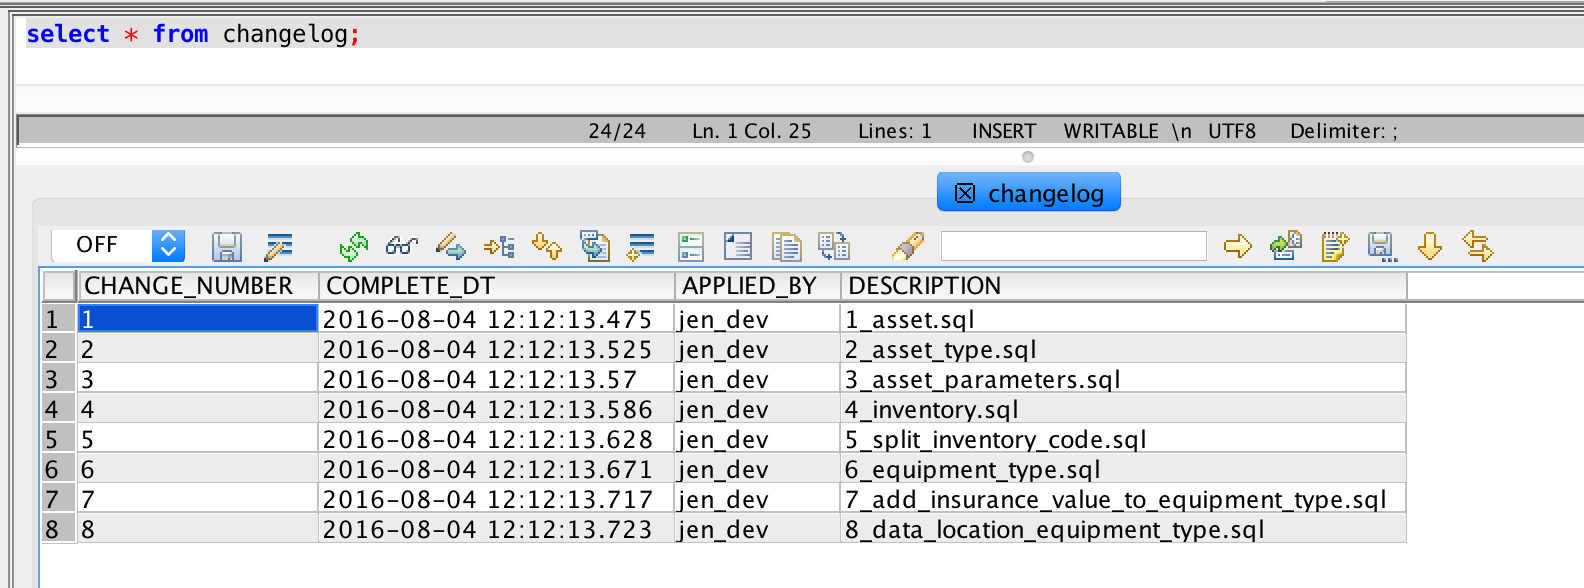
\includegraphics[width=0.95\textwidth]{changelog_screen}
  \end{center}
  \caption{changelog table maintained by database migration frameworks}
  \label{fig:db-changelog}
\end{figure}

With this numbering scheme in place, we can then track changes as they
apply to the many databases that we manage.

\begin{figure}[H]
  \begin{center}
    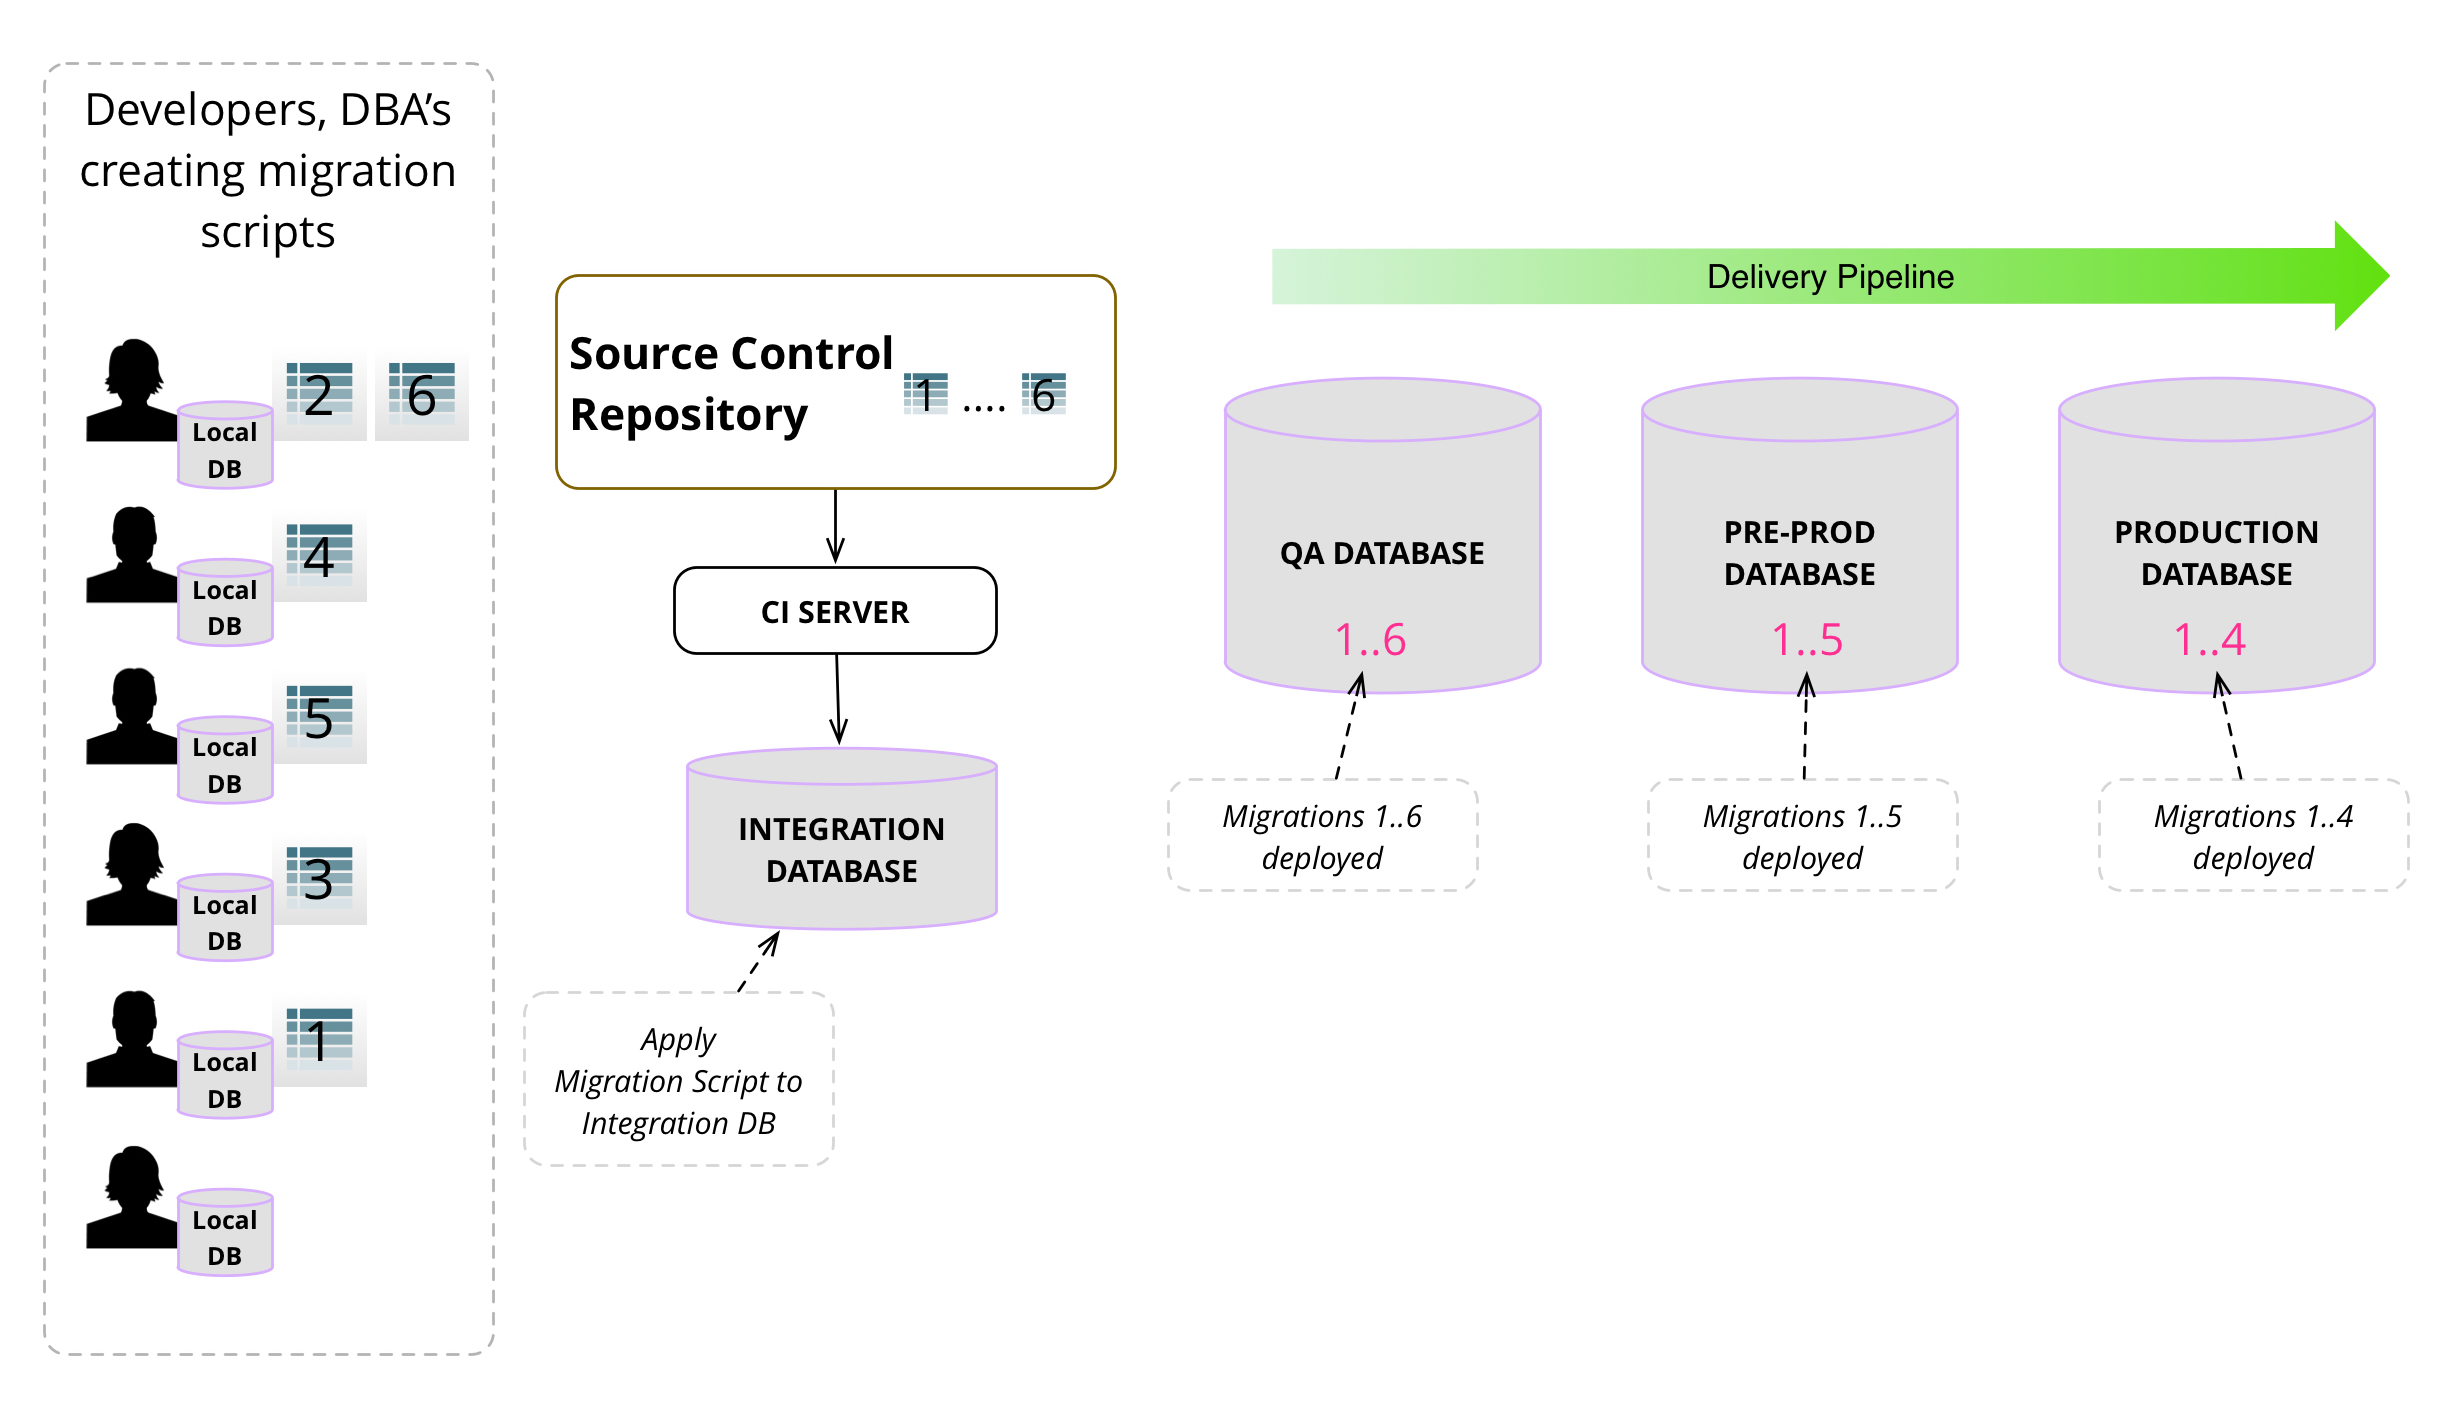
\includegraphics[width=0.95\textwidth]{migrations_lifecycle}
  \end{center}
  \caption{Life of a migration script from its creation to its deployment in production}
  \label{fig:migration-lifecycle}
\end{figure}

Some of these data migrations may have to be released more frequently
than the migrations related to new features, in that scenario, we have
found it to be useful to have separate migration repository or folder
for data related bug fixes.

\begin{figure}[H]
  \begin{center}
    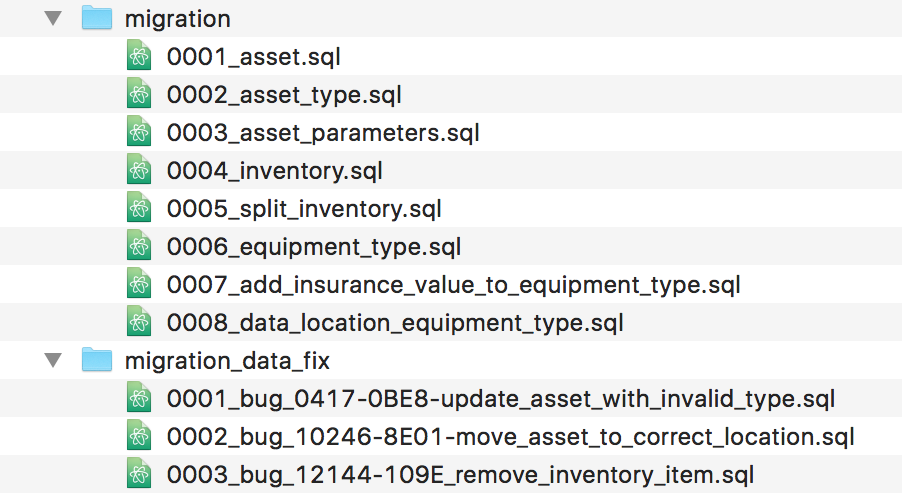
\includegraphics[width=0.95\textwidth]{seperate_data_migration_folder}
  \end{center}
  \caption{Separate folders to manage new feature database changes and production data fixes}
  \label{fig:seperate-data-migration-folder}
\end{figure}

Each of these folders can be tracked separately by the database
migration tools such as \href{http://flywaydb.org/}{Flyway},
\href{http://dbdeploy.com/}{dbdeploy},
\href{https://github.com/mybatis/migrations}{MyBatis} or similar tools,
with a separate table to store the migration numbers. The property
flyway.table in Flyway is used to change the name of the table where the
migration metadata is stored

\subsection{Everybody gets their own database instance}

Most development organizations share a single development database,
which is used by all members of the organization. Perhaps a separate
database is used for QA or staging, but the notion is to limit how many
databases are running live. Sharing databases like this is a consequence
of database instances being difficult to set up and manage, leading
organizations to minimize how many there are. Controls on who can alter
the schema in such situations varies, some places require all changes to
be made through the DBA team, others allow any developers to change the
schema of the development database, and the DBAs get involved when
changes are promoted downstream.

When we started work with agile database projects, we noted that
application developers usually follow a pattern where they work in a
private working copy of the code. People learn by trying things out, so
in programming terms developers experiment with how to implement a
certain feature and may make a few attempts before picking one. It's
important to be able to experiment in private workspace and pushing to a
shared area when things are more stable. If everyone is working in a
shared area, then they are constantly interrupting each other with
half-done changes. Although we favor Continuous Integration, where
integrations occur after no more than a few hours, the private working
copy is still important. Version control systems support this work,
allowing developers to work independently while supporting integrating
their work in a mainline copy.

This separate working works with files, but it can also work with
databases. Each developer gets their own database instance which they
can freely modify without touching other people's work. When they are
ready they can push and share their changes, as we'll see in the next
section.

These separate databases can either be separate schemas on a shared
server or, more commonly these days, a separate database running on a
developer's laptop or workstation. A decade ago, database licensing
costs could make individual database instances prohibitively expensive -
but these days this is rarely the case, particularly as open-source
databases have grown in popularity. We've found it handy to run a
database in a virtual machine running on a developer's machine. We
define the build of the database VM using
\href{https://www.vagrantup.com}{Vagrant} and
\href{https://martinfowler.com/bliki/InfrastructureAsCode.html}{Infrastructure
As Code}, so the developer doesn't need to know the details of setting
up the database VM, or have to do it manually.

\begin{figure}[H]
  \begin{center}
    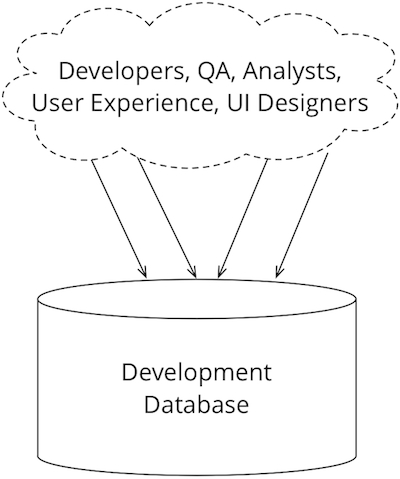
\includegraphics[width=0.35\textwidth]{single_database_problem}
  \end{center}
  \caption{Problem using a single database schema for all members on the team in development}
  \label{fig:single-database-problem}
\end{figure}

\begin{figure}[H]
  \begin{center}
    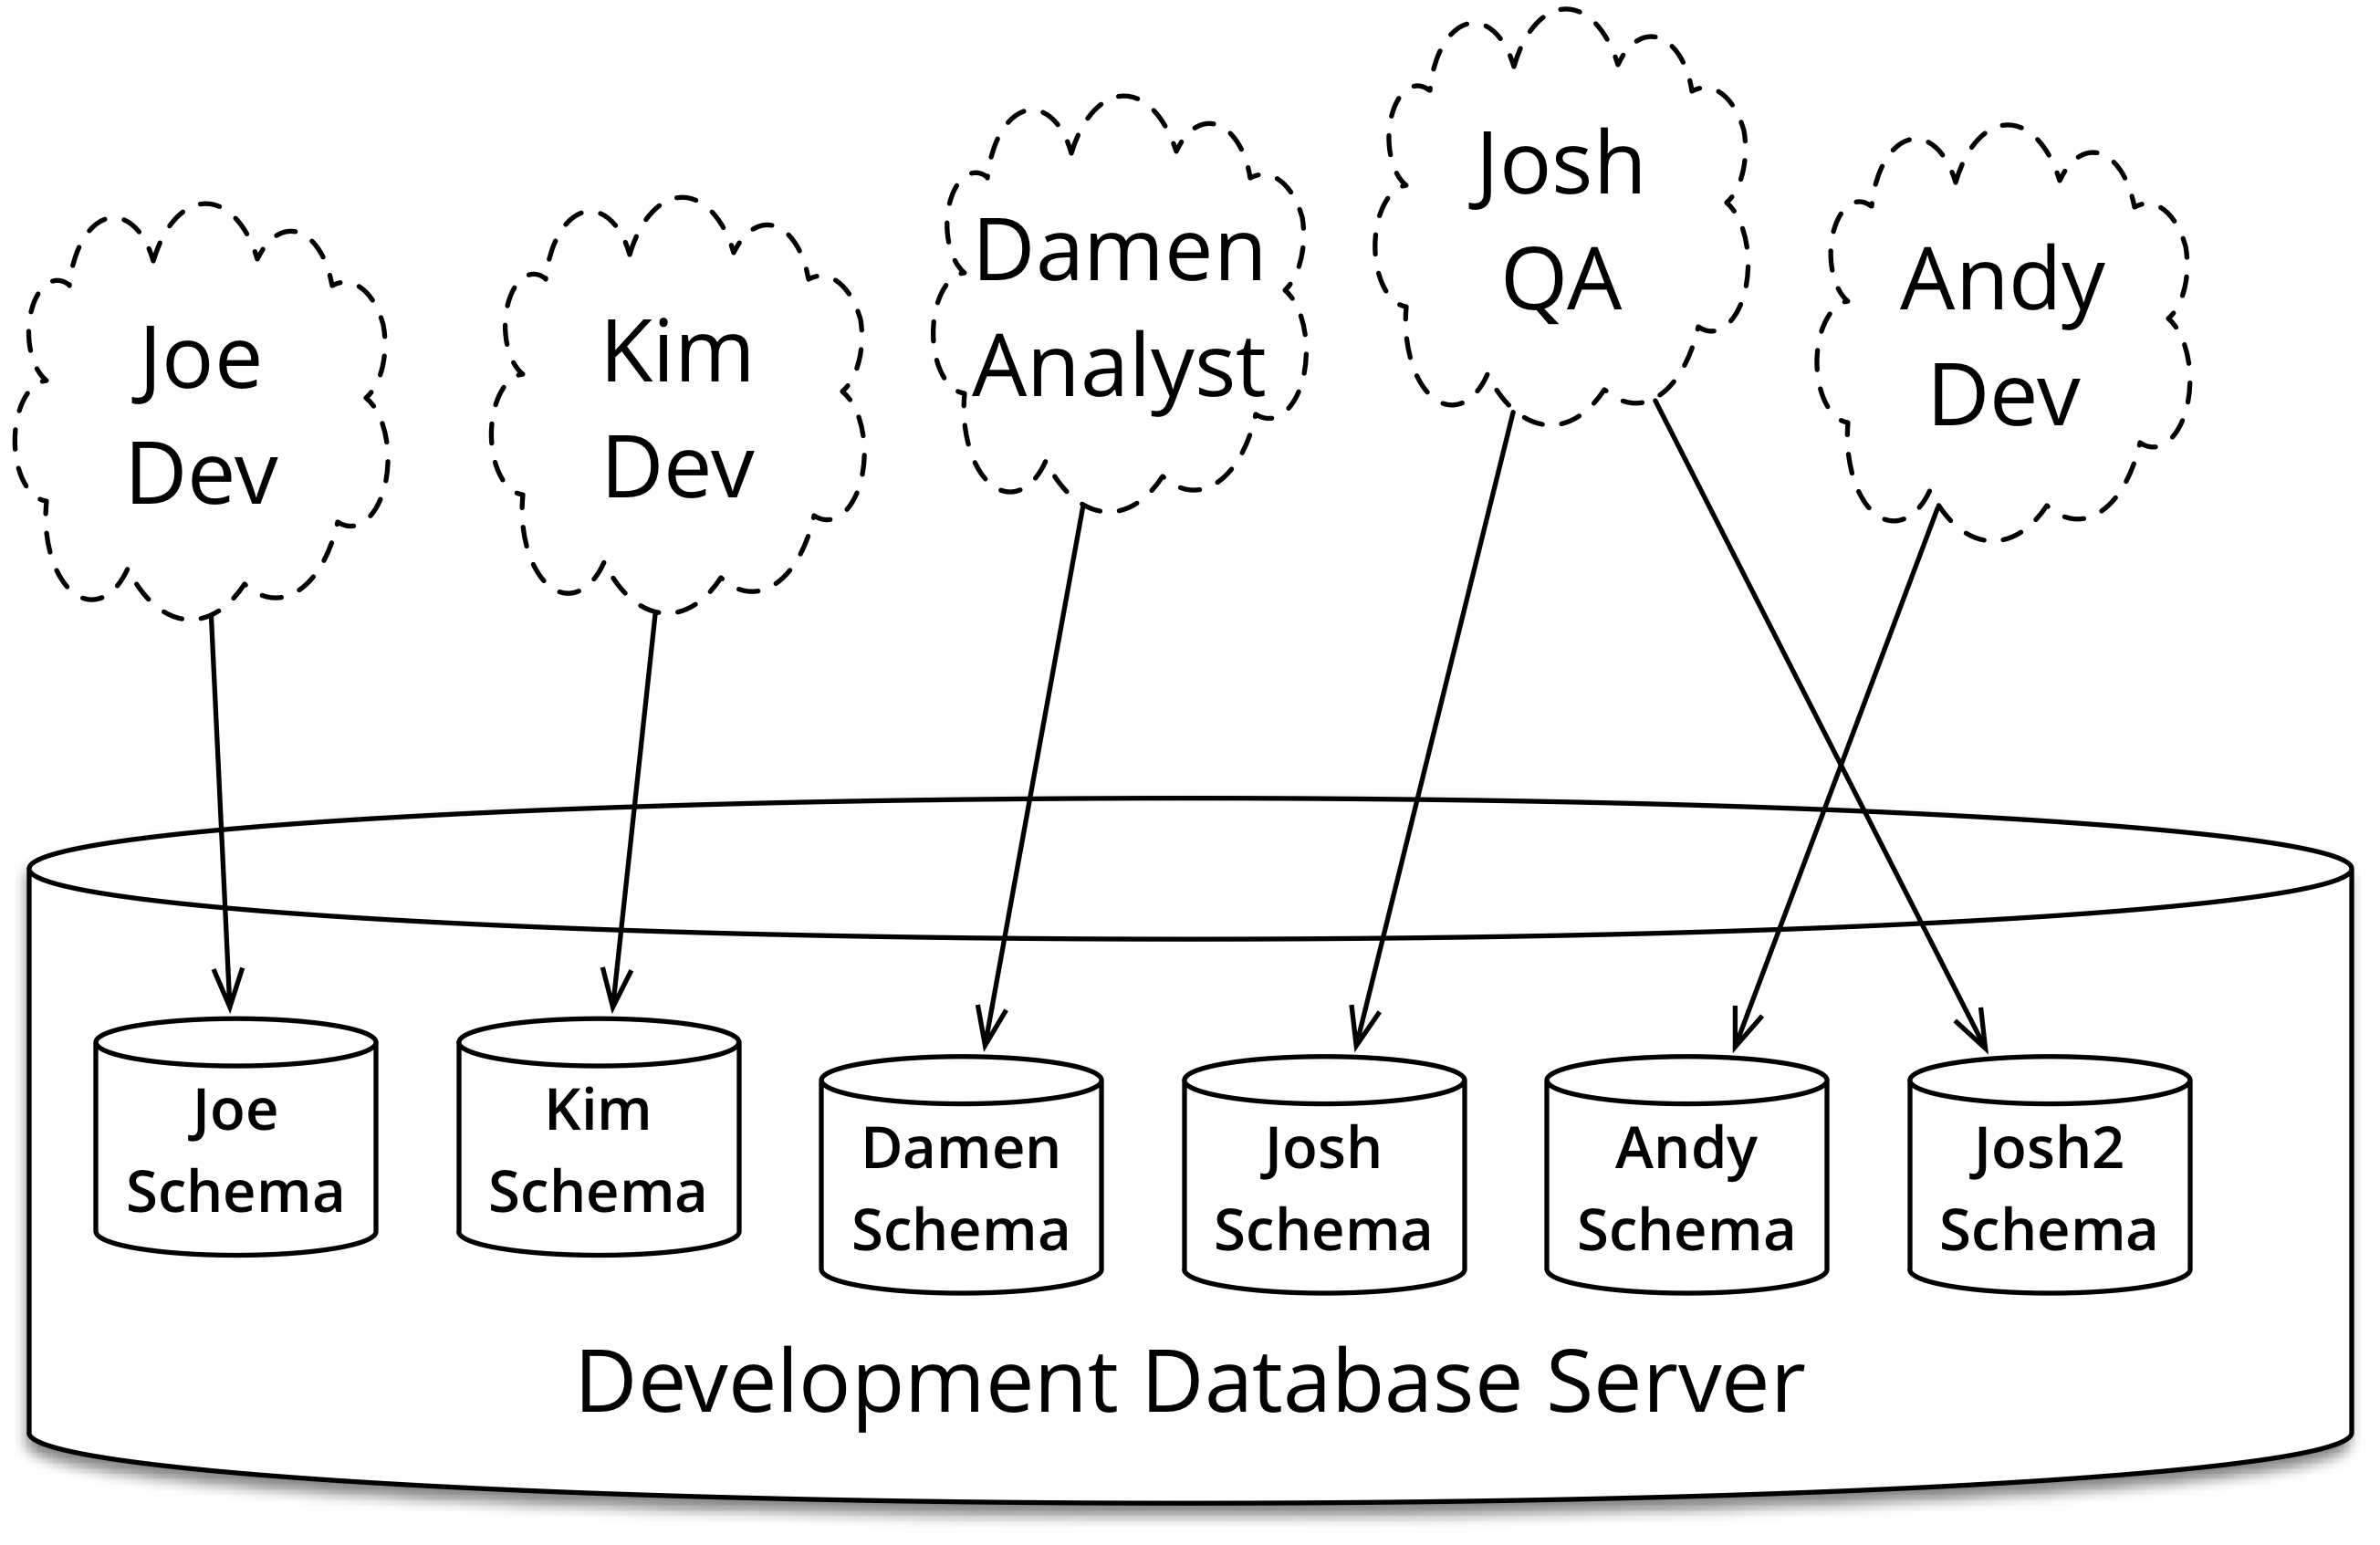
\includegraphics[width=0.95\textwidth]{multiple_database_for_everyone}
  \end{center}
  \caption{Every member of the team gets their own database schema for development and testing}
  \label{fig:multiple-database-for-everyone}
\end{figure}

Many DBAs still see multiple databases as anathema, too difficult to
work in practice, but we've found that you can easily manage a hundred
or so application database instances. The vital thing is to have tools
to allow you to manipulate databases much as you would manipulate files.

\begin{xmlcode}
<target name="create_schema"
        description="create a schema as defined in the user properties">
    <echo message="Admin UserName: ${admin.username}"/>
    <echo message="Creating Schema: ${db.username}"/>
    <sql password="${admin.password}" userid="${admin.username}"
         url="${db.url}" driver="${db.driver}" classpath="${jdbc.classpath}"
         >
        CREATE USER ${db.username} IDENTIFIED BY ${db.password} DEFAULT TABLESPACE ${db.tablespace};
        GRANT CONNECT,RESOURCE, UNLIMITED TABLESPACE TO ${db.username};
        GRANT CREATE VIEW TO ${db.username};
        ALTER USER ${db.username} DEFAULT ROLE ALL;
    </sql>
</target>
\end{xmlcode}

Creation of developer schemas can be automated, using the build script
to reduce workload on the DBA. This automation can also be restricted
just to environments in development.

\begin{xmlcode}
<target name="drop_schema">
    <echo message="Admin UserName: ${admin.username}"/>
    <echo message="Working UserName: ${db.username}"/>
    <sql password="${admin.password}" userid="${admin.username}"
         url="${db.url}" driver="${db.driver}" classpath="${jdbc.classpath}"
         >
        DROP USER ${db.username} CASCADE;
    </sql>
</target>
\end{xmlcode}

For example, a developer joins a project, checks out the code base and
starts to setup her local development environment. She uses the template
build.properties file and makes changes, such as setting db.username to
Jen and so forth for the rest of the settings. Once these settings are
done she can just run ant \verb=create_schema= and get a schema of her own on
the team development database server or database server on his laptop.

With the schema created, she can then run the database migration script
to build all the database content to populate her database instance:
tables, indexes, views, sequences, stored procedures, triggers, synonyms
and other database specific objects.

Similarly, there are scripts to delete schemas - either because they are
no longer needed, or merely because the developer wishes to clean up and
start again with a fresh schema. Database environments should be
phoenixes - regularly burnt down and rebuilt at will. That way there's
less danger of environments accumulating characteristics that aren't
reproducible, or audited.

This need for a private workspace is true for developers, but also true
for everyone else on the team. QA staff should create their own
databases, so they also can work without danger of getting confused by
changes outside their knowledge. DBAs should be able to experiment with
their own database copy as they explore modeling options, or performance
tuning.

\subsection{Developers continuously integrate database changes}

Although developers can experiment frequently in their own sandbox, it's
vital to integrate their different changes back together frequently
using
\href{https://martinfowler.com/articles/continuousIntegration.html}{Continuous
Integration (CI)}. CI involves setting up an integration server that
automatically builds and tests the mainline software. Our rule of thumb
is that each developer should integrate into mainline at least once a
day. Many tools exist to help with CI including:
\href{https://www.gocd.org/}{GoCD}, \href{https://snap-ci.com/}{Snap
CI}, \href{https://jenkins.io/}{Jenkins},
\href{https://www.atlassian.com/software/bamboo}{Bamboo} and
\href{https://travis-ci.com/}{Travis CI}

\begin{figure}[H]
  \begin{center}
    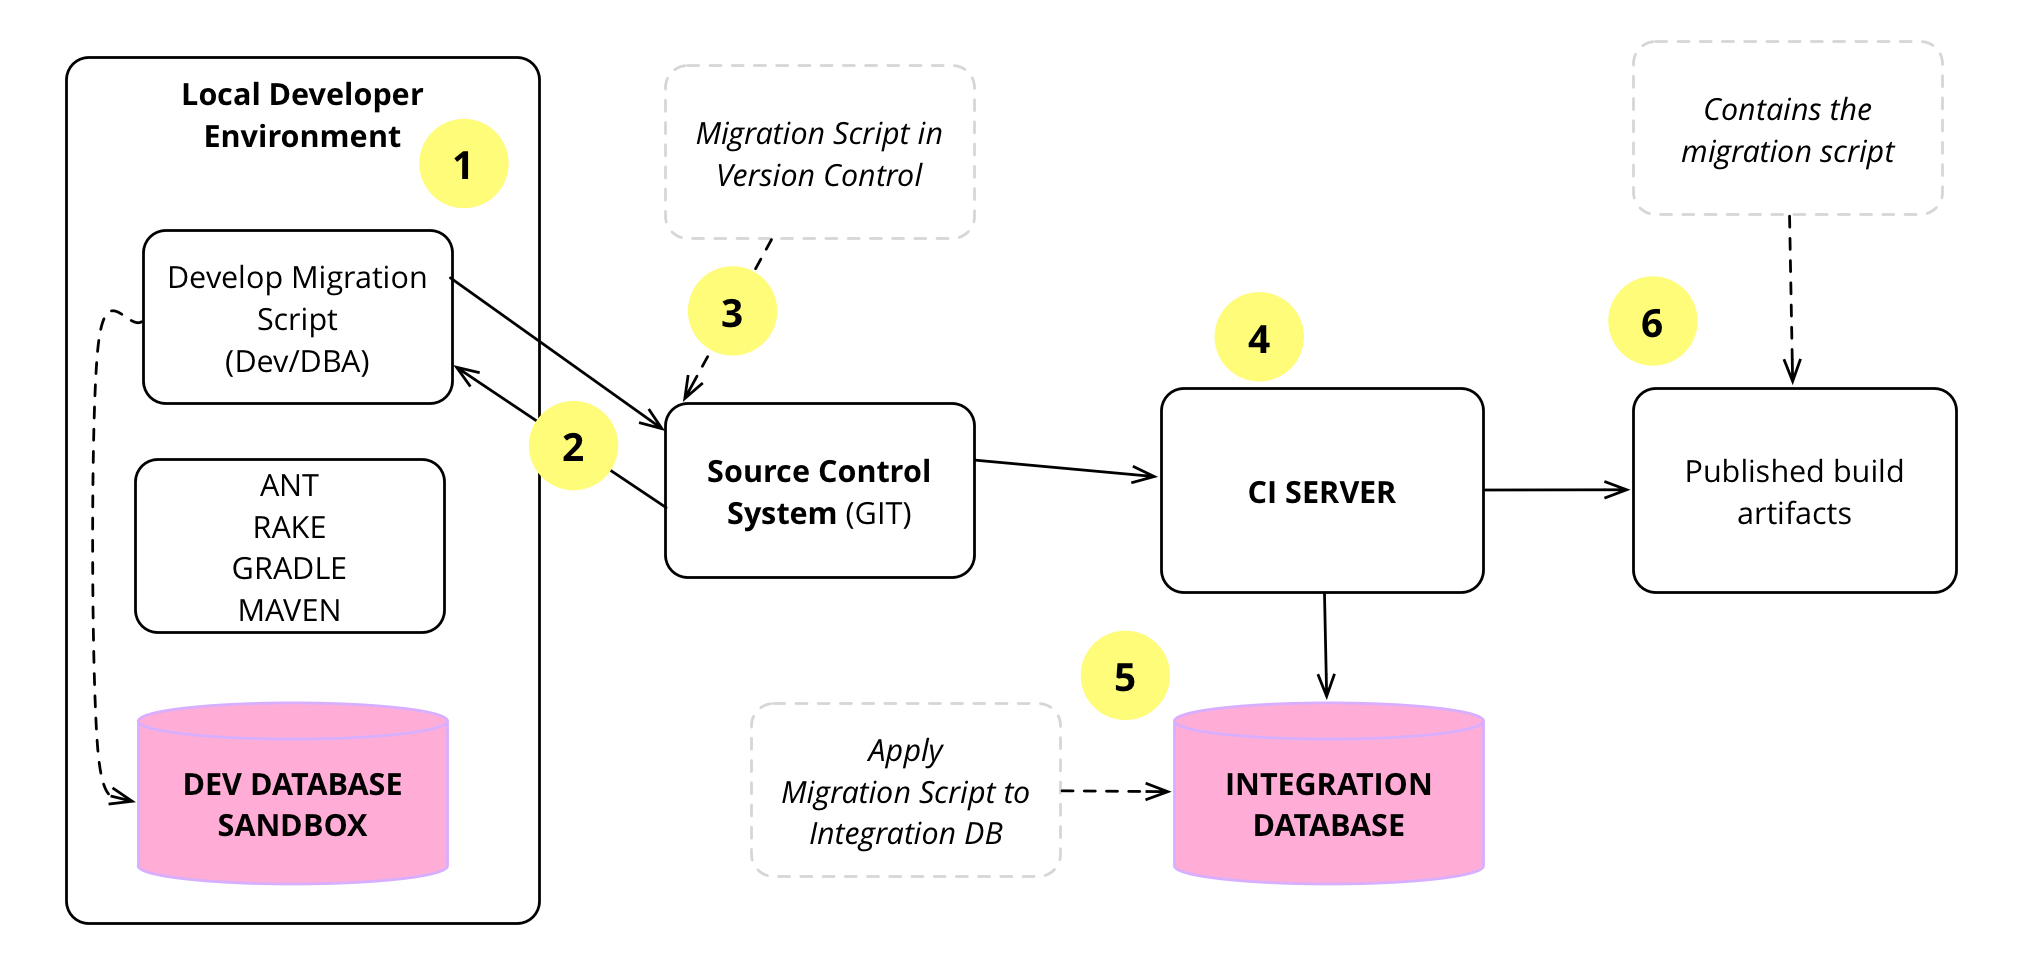
\includegraphics[width=0.95\textwidth]{ciworkflow}
  \end{center}
  \caption{Database changes, migrations being developed and integrated just like application code}
  \label{fig:ciworkflow}
\end{figure}

Figure \ref{fig:ciworkflow} shows the flow of how database migrations are
developed, tested locally, checked into source control, picked up by the
CI server and applied to the integration database, tested again, and
packaged for downstream use.

Let's take an example

\begin{enumerate}
  \item Jen starts a development that include a database schema change.
    If the change is easy, such as adding a column, Jen decides how to
    make the change directly. If it's complicated she grabs the DBA and
    talks it over with her.

    Once she has sorted out the change, she writes the migration.
    \begin{sqlcode}
ALTER TABLE project ADD projecttypeid NUMBER(10) NULL;

ALTER TABLE project ADD (CONSTRAINT fk_project_projecttype
  FOREIGN KEY (projecttypeid)
  REFERENCES projecttype DEFERRABLE INITIALLY DEFERRED)
;

UPDATE project
   SET projecttypeid = (SELECT projecttypeid
                          FROM projecttype
                         WHERE name='Integration'
                        )
;
    \end{sqlcode}

        Adding a nullable column is a backwards compatible change, so
        she can integrate the change without needing to change any
        application code. However, if it isn't a backwards compatible
        change, such as splitting a table, then Jen would need to modify
        the application code too.

      \item Once Jen has finished her changes, she is ready to
        integrate. The first step in integration is updating her local
        copy from mainline. These are changes other members of the team
        have done while she's been working on her task. She then checks
        her changes work with these updates by rebuilding the database
        and running all the tests.

        If she runs into problems, due to the other developers’ changes
        interfering with hers, she needs to fix those problems on her
        copy. Usually such clashes are easy to sort out, but
        occasionally they are more involved. Often these more complex
        conflicts trigger a conversation between Jen and her teammates
        so they can sort out how to resolve overlapping changes.

        Once she has her local copy working again, she checks to see if
        any more changes have been pushed to master while she's working,
        if so she needs to repeat the integration with the new changes.
        Usually, however, it doesn't take more than one or two of these
        cycles before her code is fully integrated with mainline.

      \item Jen pushes the change to mainline. Since the change is
        backwards compatible with the existing application code, she can
        integrate the database change before updating the application
        code to use it - a common example of Parallel Change.

      \item The CI server detects the change in mainline and starts a
        new build which contains the database migration.

      \item The CI server uses its own database copy for the build, so
        applies the database migration script to this database to apply
        the changes in the migration. In addition it runs the rest of
        the build steps: compile, unit tests, functional tests etc.

      \item Once the build finishes successfully, the CI server packages
        the build artifacts and publishes them. These build artifacts
        contain the database migration scripts, so that they can be
        applied to the databases in downstream environments, such as a
        \href{https://martinfowler.com/bliki/DeploymentPipeline.html}{Deployment
        Pipeline}. The build artifacts also contain the application code
        packaged into a jar, war, dll etc.

\end{enumerate}

This is exactly the practice of
\href{https://martinfowler.com/articles/continuousIntegration.html}{Continuous
Integration}, which is commonly used with application source code
management. The steps above are just about treating the database code as
another piece of source code. As such the database code - DDL, DML,
Data, views, triggers, stored procedures - is kept under configuration
management in the same way as the source code. Whenever we have a
successful build, by packaging the database artifacts along with the
application artifacts, we have a complete and synchronized version
history of both application and database.

With application source code, much of the pain of integrating with
changes can be handled by source code control systems and using various
tests in local environments. For databases there's a bit more effort
involved as there is data (state) in the database that needs to preserve
its business meaning. (We'll talk more about automated database
refactorings like this shortly.) In addition the DBA needs to look at
any database changes and ensure that they fit within the overall scheme
of the database schema and data architecture. For all this to work
smoothly, big changes shouldn't come as surprises at integration time -
hence the need for the DBA to collaborate closely with the developers.

We emphasize integrating frequently because we've found that it's much
easier to do frequent small integrations rather than infrequent large
integrations - a case of
\href{https://martinfowler.com/bliki/FrequencyReducesDifficulty.html}{Frequency
Reduces Difficulty}. The pain of integration increases exponentially
with the size of the integration, so doing many small changes is much
easier in practice, even though it appears counter-intuitive to many.

\subsection{A database consists of schema and data}

When we talk about a database here, we mean not just the schema of the
database and database code, but also a fair amount of data. This data
consists of common standing data for the application, such as the
inevitable list of all the states, countries, currencies, address types
and various application specific data. We may also include some sample
test data such as a few sample customers, orders etc. This sample data
would not make it to production, unless specifically needed for sanity
testing or semantic monitoring.

This data is there for a number of reasons. The main reason is to enable
testing. We are great believers in using a large body of automated tests
to help stabilize the development of an application. Such a body of
tests is a common approach in agile methods. For these tests to work
efficiently, it makes sense to work on a database that is seeded with
some sample test data, which all tests can assume is in place before
they run.

This sample data needs to be version controlled, so we know where to
look for it when we need to populate a new database, and so we have a
record of changes that's synchronized with the tests and application
code.

As well as helping test the code, this sample test data also allows to
test our migrations as we alter the schema of the database. By having
sample data, we are forced to ensure that any schema changes also handle
sample data.

In most projects we've seen this sample data be fictional. However in a
few projects we've seen people use real data for the samples. In these
cases this data's been extracted from prior legacy systems with
automated data conversion scripts. Obviously you can't convert all the
data right away, as in early iterations only a small part of the new
database is actually built. But we can use
\href{https://martinfowler.com/bliki/IncrementalMigration.html}{Incremental
Migration} to develop the conversion scripts to provide necessary data
just in time.

Not just does this help flush out data conversion problems early, it
makes it much easier for domain experts to work with the growing system
as they are familiar with the data they are looking at and can often
help to identify cases that may cause problems for the database and
application design. As a result we are now of the view that you should
try to introduce real data from the very first iteration of your
project. We've found \href{http://jailer.sourceforge.net/}{Jailer} to be
a useful tool to help with this process.


\subsection{All database changes are database refactorings}

The changes that we make to the database alter the way the database
stores information, introduces new ways to store information, or removes
storage that's no longer needed. But none of the database changes, on
their own, change the overall behavior of the software. Consequently we
can see them as fitting the definition of a refactoring.

\begin{shadequote}[r]{-- Refactoring (chapter 2)}
  a change made to the internal structure of software to make it easier
  to understand and cheaper to modify without changing its observable
  behavior
\end{shadequote}

Recognizing this, we collected and documented many of these
refactorings. By writing such a catalog, we make it easier to make these
changes correctly since we can follow the steps we've successfully used
before.

One of the big differences about database refactorings is that they
involve three different changes that have to be done together

\begin{itemize}
  \item Changing the database schema
  \item Migrating the data in the database
  \item Changing the database access code
\end{itemize}

Thus whenever we describe a database refactoring, we have to describe
all three aspects of the change and ensure that all three are applied
before we apply any other refactorings.

Like code refactoring, database refactorings are very small. The concept
of chaining together a sequence of very small changes is much the same
for databases as it is for code. The three dimensional nature of the
change makes it all the more important to keep to small changes.

Many database refactorings, such as
\href{http://databaserefactoring.com/IntroduceNewColumn.html}{Introduce
New Column}, can be done without having to update all the code that
accesses the system. If code uses the new schema without being aware of
it, the column will just go unused. Many changes, however don't have
this property, we call these {\bfseries{destructive changes}}. Destructive
changes need a bit more care, the degree of which depends on the degree
of destruction involved.

An example of a minor destructive change is
\href{http://databaserefactoring.com/MakeColumnNonNullable.html}{Make
Column Non Nullable}, which changes a nullable column to not nullable.
This is destructive because if any existing code doesn't set it to a
value, then we'll get an error. We'll also get problems if there are any
nulls in the existing data.

We can avoid the problem with existing nulls (at the cost of slightly
different ones) by assigning default data to any rows that have nulls
here. For the problem of application code not assigning (or assigning
null) we have two options. One is to set a default value to the column.

\begin{sqlcode}
ALTER TABLE customer
  MODIFY last_usage_date DEFAULT sysdate;

UPDATE customer
  SET last_usage_date =
    (SELECT MAX(order_date) FROM order
      WHERE order.customer_id = customer.customer_id)
  WHERE last_usage_date IS NULL;

UPDATE customer
  SET last_usage_date = last_updated_date
  WHERE last_usage_date IS NULL;

ALTER TABLE customer
  MODIFY last_usage_date NOT NULL;
\end{sqlcode}

The other way of dealing with a lack of assignment is to change the
application code as part of the refactoring. This is the option we
prefer if we can confidently get to all the code that updates the
database, which is usually easy if the database is only used by a single
application, but is hard if it's a shared database.

A more complex case is
\href{http://databaserefactoring.com/SplitTable.html}{Split Table},
particularly if the access to the table is spread widely across the
application code. If this is the case it's important to let everyone
know that the change is coming up so they can prepare themselves for it.
It may also be wise to wait for a relatively quiet moment, such as the
start of an iteration.

Any destructive change is much easier if database access is all
channeled through a few modules of the system. That makes it easier to
find and update the database access code.

The important thing overall is to choose a procedure that's appropriate
for the kind of change that you're making. If in doubt try to err on the
side of making changes easier. Our experience is that we got burned much
less frequently than many people would think, and with a strong
configuration control of the entire system it's not difficult to revert
should the worst happen.

Taking care of database changes including DDL, DML and data migration
during development, provides the most context for the data team,
avoiding batch migration of all changes by data team during deployment
without context.

\subsubsection{Transition phase}

We've already alluded to the difficulties we run into when we get a
destructive database refactoring and we can't easily change the access
code. These problems grow horns and big sharp teeth when you have a
shared database, which may have many applications and reports using it.
In this situation, you have to take much more care over something like a
\href{http://databaserefactoring.com/RenameTable.html}{Rename Table}. To
keep us safe from such horns and teeth, we turn to the transition phase.

A {\bfseries transition phase} is a period of time when the database
supports both the old access pattern and the new ones simultaneously.
This allows older systems time to migrate over to the new structures at
their own pace.

\begin{figure}[H]
  \begin{center}
    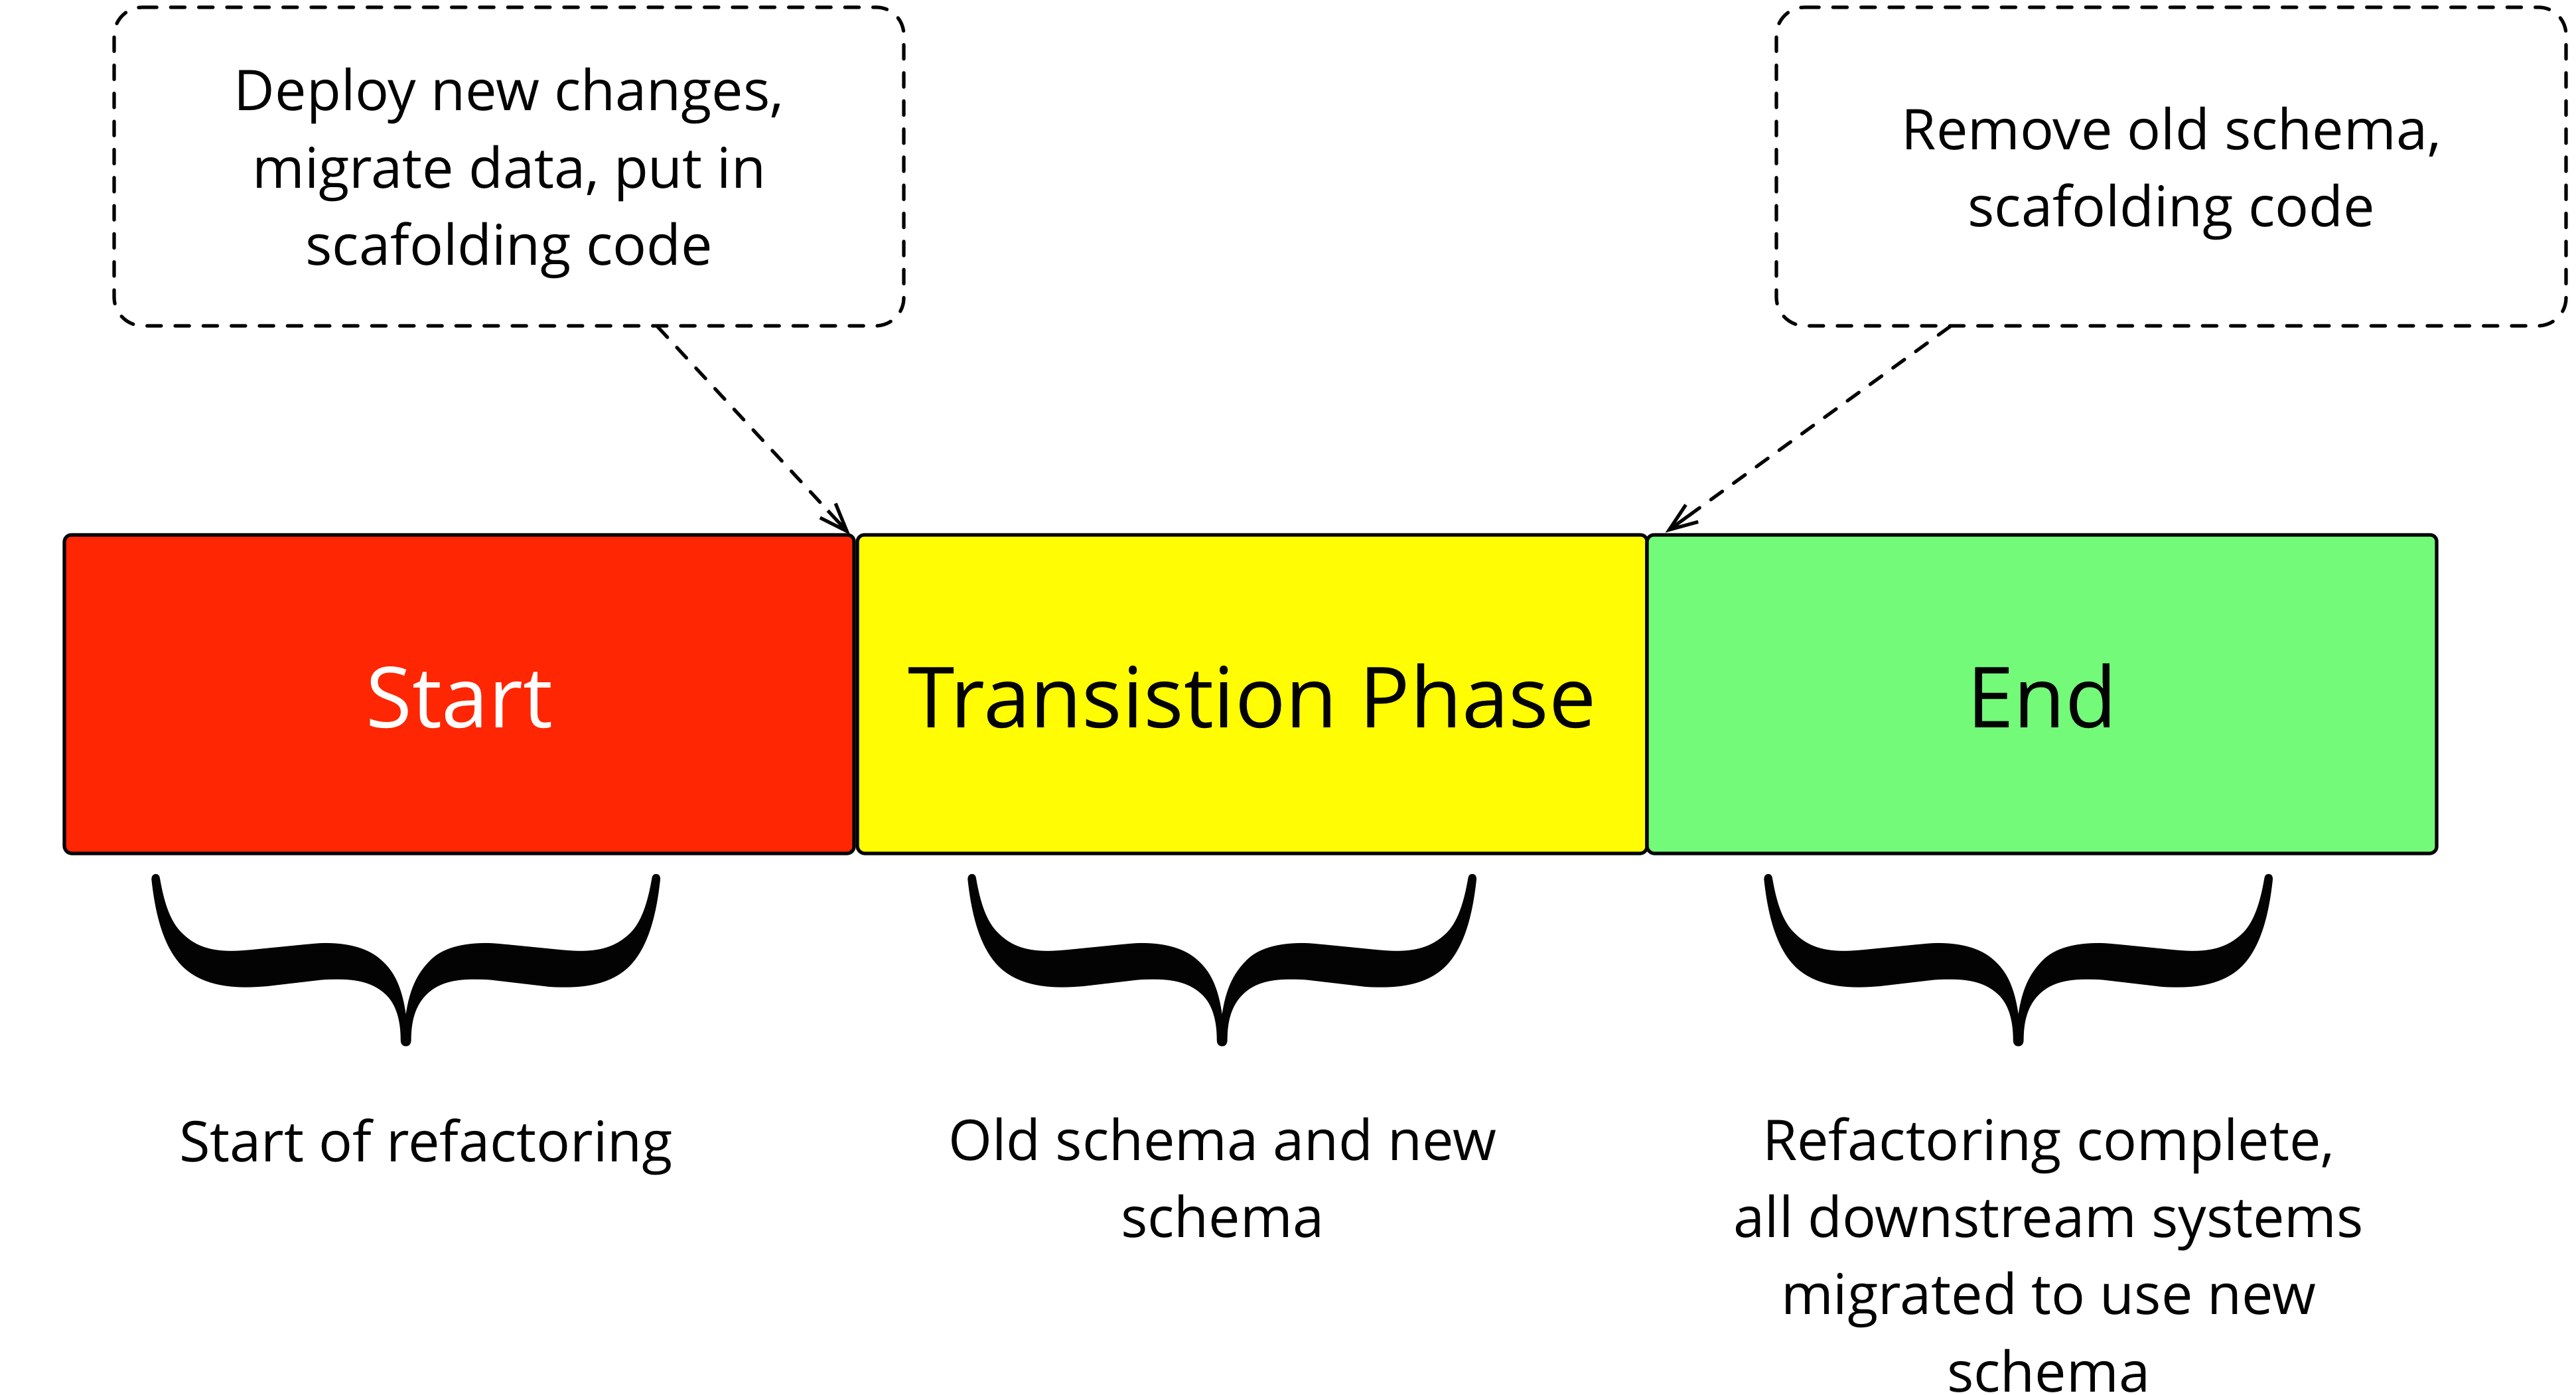
\includegraphics[width=0.95\textwidth]{stages_refactoring}
  \end{center}
  \caption{Database refactorings, being applied to legacy database and the phases it needs to take before being implemented}
  \label{fig:stages-refactoring}
\end{figure}


\begin{sqlcode}

ALTER TABLE customer RENAME to client;

CREATE VIEW customer AS
SELECT id, first_name, last_name FROM client;
\end{sqlcode}

For the \href{http://databaserefactoring.com/RenameTable.html}{Rename
Table} example, the developer would create a script that renames the
table customer to client and also creates a view named customer that
existing applications can use. This
\href{https://martinfowler.com/bliki/ParallelChange.html}{Parallel
Change} supports new and old access. It does add complexity, so it's
important that it gets removed once downsteam systems have had time to
migrate. In some organizations this can be done in a couple of months
and in some other organizations it may take years.

Views are one technique to enable transition phases. We also make use of
database triggers, which are handy for things like
\href{http://databaserefactoring.com/RenameColumn.html}{Rename Column}

\subsection{Automate the refactorings}

Since refactoring became well known for application code, many languages
have seen good support for automated refactorings. These simplify and
speed up refactoring by swiftly carrying out the various steps with no
human involved to make mistakes. Such automation is also available for
databases. Frameworks like \href{http://liquibase.org}{Liquibase} and
\href{http://guides.rubyonrails.org/active_record_migrations.html}{Active
Record Migrations} provide a DSL to apply database refactorings,
allowing a standard way to apply database migrations.

However these kinds of standardized refactorings don't work so well for
databases since the rules for dealing with data migration and legacy
data are very dependent on a team's specific context. So we prefer to
handle database refactoring by writing scripts for migration and focus
on tools to automate how to apply them.

We write each script, as we've shown so far, by combining SQL DDL (for
the schema change) and DML (for the data migration) and putting the
result in a folder in our version-controlled repository. Our automation
ensures we never apply these changes manually, they are only applied by
the automation tooling. That way we maintain the ordering of the
refactorings and update the database metadata.

We can apply the refactorings to any database instance, to bring them up
to date with the latest master, or to any previous version. The tooling
uses the metadata information in the database to find out its current
version, then applies each refactoring between it and the desired
version. We can use this approach to update development instances, test
instances, and production databases.

Updating production databases isn't any different to test databases, we
run the same set of scripts against different data. We do prefer
releasing frequently as that keeps the updates small, as that means that
the updates occur more quickly and it is easier to deal with any
problems that come up. The easiest way to do these updates is to take
the production database down while we apply the updates, this works well
for most situations. If we have to do them while keeping the application
live, it is possible, but the techniques we use will need another
article to explain.

So far, we've found that this technique has worked remarkably well. By
breaking down all the database changes into a sequence of small, simple
changes; we've been able to make quite large changes to production data
without getting ourselves in trouble.

As well as automating the forward changes, you can consider automating
reverse changes for each refactoring. If you do this you'll be able to
back out changes to a database in the same automated way. We haven't
found this to be cost effective and beneficial enough to try all the
time, also we've not had much demand for it, but it's the same basic
principle. On the whole we prefer to write our migrations so that the
database access section can work with both the old and new version of
the database. This allows us to update the database to support a future
need and make it live, have it running in production for a while, and
then only push the update that uses the new data structures once we've
found they have settled down without problems.

These days there are many tools that automate applying database
migrations, including: \href{http://flywaydb.org}{Flyway},
\href{http://liquibase.org}{Liquibase},
\href{https://github.com/mybatis/migrations}{MyBatis migrations},
\href{http://dbdeploy.com}{DBDeploy}. Here's applying a migration with
Flyway.

\begin{bashcode}
psadalag:flyway-4 $ ./flyway migrate
Flyway 4.0.3 by Boxfuse

Database: jdbc:oracle:thin:@localhost:1521:xe (Oracle 11.2)
Successfully validated 9 migrations (execution time 00:00.021s)
Creating Metadata table: "JEN_DEV"."schema_version"
Current version of schema "JEN_DEV": << Empty Schema >>
Migrating schema "JEN_DEV" to version 0 - base version
Migrating schema "JEN_DEV" to version 1 - asset
Migrating schema "JEN_DEV" to version 2 - asset type
Migrating schema "JEN_DEV" to version 3 - asset parameters
Migrating schema "JEN_DEV" to version 4 - inventory
Migrating schema "JEN_DEV" to version 5 - split inventory
Migrating schema "JEN_DEV" to version 6 - equipment type
Migrating schema "JEN_DEV" to version 7 - add insurance value to equipment type
Migrating schema "JEN_DEV" to version 8 - data location equipment type
Successfully applied 9 migrations to schema "JEN_DEV" (execution time 00:00.394s).
psadalag:flyway-4 $ 
\end{bashcode}

\subsection{Developers can update their databases on demand}

As we explained above, the first step in integrating our changes into
mainline is pulling any changes that have occurred while we were doing
our own bit of work. Not just is this essential during the integration
step, it is often useful before we're done, so we can assess the impact
of any changes we've heard our colleagues talk about. In both cases,
it's important to be able to easily pull changes from the mainline and
apply them to our local database.

We start this by pulling changes from mainline into our local workspace.
Often that's pretty simple, but sometimes we'll find that our colleagues
have pushed a migration into mainline while we've been working. If we
have written a migration with the sequence number 8, we'll see another
migration with that number appear in our migrations folder. Running our
migration tool should detect this

\begin{bashcode}
psadalag:flyway-4 $ ./flyway migrate
Flyway 4.0.3 by Boxfuse

Database: jdbc:oracle:thin:@localhost:1521:xe (Oracle 11.2)
ERROR: Found more than one migration with version 8
Offenders:
-> /Users/psadalag/flyway-4/sql/V8__data_location_equipment_type.sql (SQL)
-> /Users/psadalag/flyway-4/sql/V8__introduce_fuel_type.sql (SQL)
psadalag:flyway-4 $
\end{bashcode}

Once we see we have a clash our first step is simple, we need to
renumber our migration to 9 so it will apply on top of the new migration
on mainline. Once we've renumbered we need to test that there aren't any
conflicts between the migrations. To do this we clean out the database
and then apply all the migrations, including the new 8 and our
renumbered 9 to a blank database copy.

\begin{bashcode}
psadalag:flyway-4 $ mv sql/V8__introduce_fuel_type.sql sql/V9__introduce_fuel_type.sql
psadalag:flyway-4 $ ./flyway clean
Flyway 4.0.3 by Boxfuse

Database: jdbc:oracle:thin:@localhost:1521:xe (Oracle 11.2)
Successfully cleaned schema "JEN_DEV" (execution time 00:00.031s)
psadalag:flyway-4 $ ./flyway migrate
Flyway 4.0.3 by Boxfuse

Database: jdbc:oracle:thin:@localhost:1521:xe (Oracle 11.2)
Successfully validated 10 migrations (execution time 00:00.013s)
Creating Metadata table: "JEN_DEV"."schema_version"
Current version of schema "JEN_DEV": << Empty Schema >>
Migrating schema "JEN_DEV" to version 0 - base version
Migrating schema "JEN_DEV" to version 1 - asset
Migrating schema "JEN_DEV" to version 2 - asset type
Migrating schema "JEN_DEV" to version 3 - asset parameters
Migrating schema "JEN_DEV" to version 4 - inventory
Migrating schema "JEN_DEV" to version 5 - split inventory
Migrating schema "JEN_DEV" to version 6 - equipment type
Migrating schema "JEN_DEV" to version 7 - add insurance value to equipment type
Migrating schema "JEN_DEV" to version 8 - data location equipment type
Migrating schema "JEN_DEV" to version 9 - introduce fuel type
Successfully applied 10 migrations to schema "JEN_DEV" (execution time 00:00.435s).
psadalag:flyway-4 $
\end{bashcode}

Usually this works just fine, but occasionally we'll see a conflict -
perhaps the other developers renamed the table that we're making a
change to. In which case we need to figure out how to resolve the
conflict. Here the small size of the migrations makes it easier to spot
and deal with conflicts.

Finally once the database changes are integrated, we need to rerun the
application test suite, in case the migration we got from mainline
causes any of our tests to break.

This procedure allows us to work independently for short periods, even
without a network connection, and then integrate whenever it suits us.
It is entirely up to us when and how often we do this integration - as
long as we ensure we are synchronized before we push to mainline.

\subsection{Clearly separate all database access code}

To understand the consequences of database refactorings, it's important
to be able to see how the database is used by the application. If SQL is
scattered willy-nilly around the code base, this is very hard to do. As
a result it's important to have a clear database access layer to show
where the database is being used and how. To do this we suggest
following one of the data source architectural patterns from
\href{https://martinfowler.com/books/eaa.html}{P ofEAA}.

Having a clear database layer has a number of valuable side benefits. It
minimizes the areas of the system where developers need SQL knowledge to
manipulate the database, which makes life easier to developers who often
are not particularly skilled with SQL. For the DBA it provides a clear
section of the code that he can look at to see how the database is being
used. This helps in preparing indexes, database optimization, and also
looking at the SQL to see how it could be reformulated to perform
better. This allows the DBA to get a better understanding of how the
database is used.

\subsection{Release frequently}

When we wrote the original version of this article over a decade ago,
there was little support for the idea that software should be frequently
released to production. Since then the rise of the internet giants has
shown that a rapid sequence of releases is a key part of a successful
digital strategy.

With every change captured in a migration, we can easily deploy new
changes into test and production environments. The kind of evolutionary
database design we discuss here is both a vital part of enabling
frequent releases, and also benefits from the learning we get from the
feedback of seeing software used for real.

\section{Variations}

Like any set of practices, these should be varied depending on your
specific circumstances, here are some of those we've encountered.

\subsection{Multiple versions}

A simple project can survive with just a single code line, and thus a
single database version. With more complex projects there's a need to
support multiple versions for AB testing, or rolling deployments when
doing \href{https://martinfowler.com/bliki/CanaryRelease.html}{Canary
Releases} and thus multiple varieties of the project database. Each
release may need its own test data, or changes to test specific feature
or fix particular bugs. This is no different than managing multiple
versions of code in production, but with the added twist that the
database has to support multiple releases of the application.

Another method we have found to be useful, is to have a single
repository for the database and all the other application versions
depend on the database repository. Using this method, you have to ensure
that all versions of the code work with the same database version, hence
forcing your database to be backwards compatible with all previous
application releases that are live in production.

\subsection{Shipping changes with application}

In some projects we have seen that the changes to the product have to be
shipped to thousands of end customers. In these kinds of projects its
better to allow the application upgrade itself by packaging all the
database changes along with the application (as we have no idea what
version the customer is upgrading from) and let the application upgrade
the database on startup using frameworks like Flyway or one of its many
cousins.

\subsection{Multiple applications using the same database}

In many enterprises, many applications end up using the same database -
the
\href{http://enterpriseintegrationpatterns.com/SharedDataBaseIntegration.html}{Shared
Database integration pattern}. In these situations, when one application
makes a change to the database, it’s quite likely that the change will
break other applications. To deal with this it’s better to extract the
database as a separate code repository which is used by all the
dependent applications. This common database repository should have
\href{http://sadalage.com/blog/2015/08/16/behavior-driven-database-development}{automated
behavior tests} which ensure that cross application dependencies are
tested, failing the build if dependent applications are affected. This
is not different than having a shared software component with its own
code repository. The software component is tested for its own view of
its behavior, but also for the contract it makes with downstream
applications using Consumer-Driven Contracts

\subsection{NoSQL Databases}

We've written this article focusing on relational databases, partly
because that's how we wrote the original, and partly since we still find
they are the most common. But we're also
\href{https://martinfowler.com/books/nosql.html}{somewhat familiar with
NoSQL databases}, which have become more common of late. A full
discussion of how to handle these in an evolutionary way would be
another article, but we will attempt a superficial overview.

NoSQL databases claim to be much easier to handle in an evolutionary way
as most of them are “schemaless”. But being schemaless doesn't free us
from worrying about schemas,
\href{https://martinfowler.com/articles/schemaless/}{there is still an
implicit schema} - one that's implied by any code that accesses the
database. That schema still has to be managed, essentially by using the
same techniques of data migrations managed in the source code
repository. The lack of a storage schema does allow us another
technique, supporting multiple read strategies for different versions.
This can make it easier to manage the evolution of databases, but it is
still something we need to worry about.

\section{You don't need an army of DBAs}

Using the techniques we describe here may sound like it is a lot of
work, but in fact it doesn't require a huge amount of people. On many
projects we have had thirty-odd developers and a team size (including,
QA, analysts and management) of close to a hundred. On any given day we
would have a hundred or so copies of various schemas out on people's
workstations. Yet all this activity needed only one full time DBA with a
couple of developers understanding the workings of the process and
workflow doing some part-time assistance and cover.

On smaller projects even that isn't needed. We've been using these
techniques on smaller projects (about a dozen people) and we find these
projects don't need a full time DBA. Instead we rely on a couple of
developers with an interest in DB issues who handle the DBA tasks
part-time and, if needed, involve a DBA to make design/architecture
decisions.

The enabler for this is automation. If you are determined to automate
every task, you can handle lot of work with much less people. Especially
with the popularity of
\href{https://martinfowler.com/bliki/DevOpsCulture.html}{DevOps} and
related tools (such as \href{https://puppetlabs.com}{Puppet},
\href{https://www.chef.io/chef}{Chef},
\href{https://www.docker.com}{Docker},
\href{https://github.com/coreos/rkt}{Rocket}, and
\href{https://www.vagrantup.com}{Vagrant}).

Since we started working in this fashion, all those years ago, we've
come to depend on databases that can be evolved just as much as
application code, allowing us to speed up release cycles and get
software into production sooner. The techniques we describe here are now
part of our habitual way of working. It's our goal, however, not just to
improve our own methods, but to share our experiences with the software
industry. The more we see techniques like these adopted, the more we see
software enabling people to fulfill their goals, producing advances that
enrich all our lives.

\section{Tools to Help}

Doing this kind of thing requires a lot of automation - here's some of
the tools we've found useful.
\begin{itemize}
  \item \href{http://liquibase.org}{Liquibase}, a framework to manage database migrations
  \item \href{https://github.com/mybatis/migrations}{MyBatis migrations}, a framework to manage database migrations
  \item \href{http://flywaydb.org}{Flyway}, a framework to manage database migrations
  \item \href{http://dbdeploy.com}{DBDeploy}, a framework to manage database migrations
  \item \href{http://www.dbmaestro.com}{DBmaestro}, a commercial tool to enable evolutionary database development
  \item \href{http://www.red-gate.com/products/dlm/dlm-automation-suite}{RedGate}, a commercial tool to enable evolutionary database development
  \item \href{http://www.datical.com/}{Datical}, a commercial tool to enable application release process
    by automating database release management
  \item \href{http://jailer.sourceforge.net}{Jailer}, a tool to extract subsets of data from a database
  \item \href{http://www.diffkit.org}{DiffKit}, a framework to compare two sets of data and report any differences
  \item \href{http://dbunit.sourceforge.net}{DbUnit}, a JUnit extension, used in testing databases
  \item \href{http://dbfit.github.io/dbfit/index.html}{DbFit}, a tool to write readable, easy-to-maintain unit and
    integration tests for your database code.
  \item \href{https://github.com/sunitparekh/data-anonymization}{Data Anonymization}, a tool to anonymize production data for development use.
\end{itemize}

Analysts and QA folks often need to look at the test data in the
database and to be able to easily change it. For that we created an
Excel application with VBA scripts to pull data down from the database
into an excel file, allow people to edit the file, and send the data
back up to the database. Although other tools exist for viewing and
editing the contents of a database, Excel works well because so many
people are familiar with it.

Everybody on the project needs to be able to explore the database design
easily, that way they can find out what tables are available and how
they are used. Building a webapp that queries database metadata gives a
easy interface for developers, QA, analysts and anyone else who wants
it. So far we've built a simple such app as part of our project tooling.

\end{document}
% vim: set ai nu nobk expandtab ts=4 sw=2 tw=72 syntax=tex :
